%%%%%%%%%%%%%%%%%%%%%%%%%%%%%%%%%%%%%%%%%%%%%%%%%%
%  Chilpancingo de los Bravos, Guerrero, México  %
%         15 noviembre del 2022 23:20            %
%      Congreso de estudiantes de Posgrado       %
%        Universidad Autónoma de Guerrero        % 
%          Plantilla Desarrollada por:           %
%          M.Sc. Camilo Mora Batista             %
%             Profesor Asistente                 %
%         Universidad de Holguín, Cuba           %
%%%%%%%%%%%%%%%%%%%%%%%%%%%%%%%%%%%%%%%%%%%%%%%%%%
\documentclass[a4paper,12pt]{article}
\usepackage[margin = 2.5cm, top =2.4cm]{geometry}
\usepackage[spanish]{babel}
\usepackage{times}
\usepackage[T1]{fontenc}
\usepackage[utf8]{inputenc}
\usepackage{plain}
\usepackage{graphicx}
\usepackage{fancyhdr}
%\usepackage{chicago} %Descomentar aqui para cambiar a estilo chicafo en las bibliografias
%\usepackage{apacite} %Descomentar aqui para cambiar a estilo APA 6ed en las bibliografia  

\fancypagestyle{plain}{
	\fancyhead[L]{\hspace{-2.5cm}
\includegraphics[scale=0.7]{leftheader2.png}}
	\fancyhead[C]{\quad\quad\vspace{1.5cm}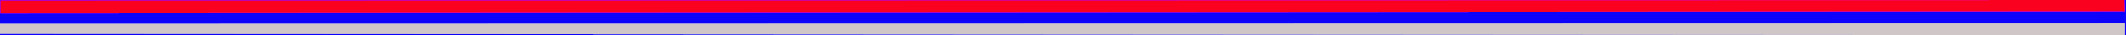
\includegraphics[width=15cm]{centerlistheadaer.jpg}}
	\fancyhead[R]{\vspace{0.5cm}\hspace{1cm}
\includegraphics[scale=0.6]{rightheader2.jpg}\hspace{-6.7cm}
\includegraphics[scale=0.11]{rightheader1.png}\qquad\qquad\quad}
	%\fancyfoot[L]{L1}
	%\fancyfoot[C]{L2}
	%\fancyfoot[R]{L3}
	\renewcommand{\headrulewidth}{0pt}
	%\renewcommand{\footrulewidth}{0.5pt}
}



%\fancyhead[L]{\includegraphics{leftheader.png}}
%\fancyhead[C]{}
%\fancyhead[R]{\thepage}
\title{Clasificación y predicción para el diagnóstico de las SCA2 a través de mediciones en Imágenes de Resonancia Magnética}

\author{José Alberto Cuesta$^1$,\underline{Camilo Mora Batista}$^2$, Cruz Vargas-de-Leon$^2$, \\ Maria Gúzman-Martínez$^2$, Frank Rodes-Carrillo$^1$, Sergio Torralbaz Fitz$^3$}

\date{}


\begin{document}
	%\vspace{-3in}
	\maketitle
	
	\begin{center}
		$ ^1$ Centro para la Investigación y Rehabilitación de las Ataxias Hereditarias, cuesta140560@gmail.com \\ 
		$^2$ Univerisdad Autónoma de Guerrero, narutokmy@gmail.com\\
		$^3$ Baptist Health South Florida. Biomedical Engineering department, torralbasfitz@gmail.com
	\end{center}
	
\section*{Resumen}
	
	La ataxia espinocerebelosa (SCA) es un término que hace referencia a un grupo de ataxias hereditarias, que son enfermedades neurológicas caracterizadas por la degeneración de las células que constituyen el cerebelo. A partir de los estudios que sugieren la Imagen por Resonancia Magnética (IRM) como un método importante que puede colaborar en el diagnóstico de las ataxias, se han investigado las mediciones lineales del Diámetro Anteroposterior del Mesencéfalo (ADM) en la IRM, correspondientes a estudios en pacientes SCA2 y Control. Para el desarrollo de la investigación se ha contado con la colaboración de 65 pacientes SCA2 y 39 pacientes Control siguiendo un criterio de inclusión y exclusión en ambos casos.  En esta ponencia se aborda un modelo de regresión logística que nos permite emitir un criterio diagnóstico sobre los pacientes con SCA2 basado en el ADM. El modelo propuesto ha sido creado con el 80\% de la muestra, validado con el 20\%. La bondad de ajuste del modelo a los datos se verificó mediante el test de Hosmer-Lemeshow. Para el proceso de validación, se analizaron la sensibilidad y la especificidad y se obtuvieron la razón de verosimilitud positiva y la razón de verosimilitud negativa más el coeficiente kappa. Estos resultados nos convencen de que tenemos un modelo favorable que contribuye al estudio de la SCA2. 
	
	
\textbf{Palabras Clave:}  Ataxia Espinocerebelosa; Regresión Logística; Imagen de Resonancia Magnética; Diámetro Anteroposterior del Cerebro Medio
\section{Introductión}
	
	
El término ataxia, que no define una enfermedad o diagnóstico específico, se refiere a un estado patológico de la coordinación del movimiento \cite{luis_velazquez_perez_ataxia_2012,almaguer-gotay_spinocerebellar_2017,wilke_neurofilaments_2020} y se utiliza para describir un trastorno de la marcha que se manifiesta por inestabilidad incoordinación y aumento de la base de sustentación como consecuencia de una disfunción a nivel del cerebelo y/o de sus vías, así como de alteraciones en la médula espinal, los nervios periféricos o una alteración de estas tres condiciones \cite{almaguer-gotay_spinocerebellar_2017}.

De todas las formas de ataxias, las más comunes y por tanto las más estudiadas son las ataxias hereditarias.  Las ataxias hereditarias autosómicas dominantes son comúnmente conocidas como ataxias espinocerebelosas (SCA) \cite{mascalchi_neuroimaging_2020,rodriguez-labrada_founder_2020,prooije_spinocerebellar_2021}. Comprenden un amplio grupo de enfermedades neurodegenerativas caracterizadas por una gran heterogeneidad clínica, patoló-gica y molecular. En la actualidad se conocen 48 formas moleculares de SCA, aunque la heterogeneidad genética observada entre ellas sugiere que al menos el 30\% de su etiología molecular está por identificar \cite{luis_velazquez_perez_ataxia_2012}. \\
Las ataxias hereditarias son un grupo de enfermedades neurológicas heredi-tarias que afectan al cerebelo, la médula espinal, las vías espinocerebelosas y, normalmente, los nervios periféricos. Globalmente, se caracterizan por un síndrome atáxico con incoordinación motora central y de las extremidades \cite{paap_standardized_2016,assistance_publique_-_hopitaux_de_paris_identification_2019}. 
Se han realizado valiosas aportaciones que actualmente permiten conocer parte de las características genéticas de al menos 28 formas moleculares de Ataxias Espinocerebelosas Autosómicas Dominantes. De las 48 formas molecu-lares conocidas de Ataxia Espinocerebelosa ( SCA); la SCA2 representa el 15\% de todas las SCA a nivel internacional, y se distribuye en gran parte del mundo, sin embargo, en Cuba constituye el 76\% de las ataxias hereditarias \cite{meira_neuroradiological_2019,bhandari_spinocerebellar_2022}, específicas en la provincia de Holguín. \\
El diagnóstico de la ataxia espinocerebelosa cuenta con la ayuda de patólogos, radiólogos, neurólogos y genetistas. Los avances en el análisis y las pruebas genéticas moleculares agilizan la clasificación y el diagnóstico precoz definitivo. La determinación de un tipo específico de ataxia puede requerir tiempo y mucho apoyo económico. Por lo tanto, la manifestación clínica y la caracteriza-ción son imperativas antes del análisis genético. Pero los fenotipos de los distintos subtipos de SCA se solapan, por lo que el genotipo se ha convertido en el patrón de oro para el diagnóstico. Sin embargo, en los casos con características fenotípicas complejas o únicas, puede ser necesaria una evaluación genética adicional que guíe las pruebas genéticas específicas del subtipo definitivo \cite{silva_diagnosis_2019}.  En los subtipos más comunes y conocidos, como SCA1, SCA2, SCA3, SCA6, SCA7, SCA8 y SCA10, también se realizan análisis de sangre para detectar mutaciones. 



El diagnóstico de la SCA requiere un estudio costoso, lo que ha llevado a la búsqueda de biomarcadores más económicos. Esto ha llevado a la aparición de diferentes tipos de escalas de evaluación para descartar subtipos de ataxia. Entre estas escalas se encuentra la ICARS que fue la primera escala de ataxia y es ampliamente utilizada en estudios observacionales así como en ensayos de intervención \cite{bhandari_spinocerebellar_2022}. Consta de 19 ítems agrupados en cuatro subescalas que contribuyen a una puntuación total de 100 puntos \cite{paap_standardized_2016}. Las subdivisiones de los diferentes componentes de la ataxia son alteraciones posturales y de la marcha, ataxia de las extremidades, disartria y trastornos oculomotores. Otra de estas escalas clínicas es la SARA, basada en una evaluación semicuantitativa de la ataxia cerebelosa. Estas son las escalas más conocidas, pero existen otras escalas que se pueden encontrar en \cite{silva_diagnosis_2019,muthuswamy_diagnosis_2013}. También se encuentran estudios de registros electrooculográficos principalmente con casos de SCA2.

La neuroimagen permite evaluar las alteraciones morfológicas y funcionales del cerebro y la médula espinal en los pacientes con ataxia. La mayoría de los estudios de neuroimagen en la ataxia utilizan la resonancia magnética, pero también hay estudios de imagen molecular con radiotrazadores. En un reciente documento de consenso se analizó la aplicación de estos métodos de neuroimagen en la ataxia \cite{oz_mr_2020,klaes_mr_2016,wan_mr_2020}.  Las neuroimágenes demuestran la atrofia cerebelosa bruta más prominente en SCA2 y menos en otros subtipos, el agrandamiento de los ventrículos y la atrofia de otras partes del cerebro también \cite{cocozza_conventional_2021,cabeza-ruiz_convolutional_2021,cabeza-ruiz_convolutional_2022,klaes_mr_2016,oz_mr_2020,mascalchi_neuroimaging_2020}. 


	
\section{Metodología}
Fue en el Concilio de Roma del año 382, cuando la Iglesia católica junto al papa Dámaso instituyeron el Canon Bíblico con la lista del Nuevo Testamento similar al de Atanasio de Alejandría y los libros del Antiguo Testamento de la Versión de los . Esta versión fue traducida del griego al latín por Jerónimo la Vulgata por encargo de la iglesia. Posteriormente los Concilios regionales de Hipona del 393,  de Cartago del 397 y IV de Cartago del 419, en los cuales participó Agustín de Hipona, aprobaron definitivamente dicho canon. En el año 405 esta lista fue enviada por Inocencio al obispo Exuperi

Fue en el Concilio de Roma del año 382, cuando la Iglesia católica junto al papa Dámaso instituyeron el Canon Bíblico con la lista del Nuevo Testamento similar al de Atanasio de Alejandría y los libros del Antiguo Testamento de la Versión de los . Esta versión fue traducida del griego al latín por Jerónimo la Vulgata por encargo de la iglesia. Posteriormente los Concilios regionales de Hipona del 393,  de Cartago del 397 y IV de Cartago del 419, en los cuales participó Agustín de Hipona, aprobaron definitivamente dicho canon. En el año 405 esta lista fue enviada por Inocencio al obispo Exuperi

Fue en el Concilio de Roma del año 382, cuando la Iglesia católica junto al papa Dámaso instituyeron el Canon Bíblico con la lista del Nuevo Testamento similar al de Atanasio de Alejandría y los libros del Antiguo Testamento de la Versión de los . Esta versión fue traducida del griego al latín por Jerónimo la Vulgata por encargo de la iglesia. Posteriormente los Concilios regionales de Hipona del 393,  de Cartago del 397 y IV de Cartago del 419, en los cuales participó Agustín de Hipona, aprobaron definitivamente dicho canon. En el año 405 esta lista fue enviada por Inocencio al obispo Exuperi

íblico con la lista del Nuevo Testamento similar al de Atanasio de Alejandría y los libros del Antiguo Testamento de la Versión de los . Esta versión fue traducida del griego al latín por Jerónimo la Vulgata por encargo de la iglesia. Posteriormente los Concilios regionales de Hipona del 393,  de Cartago del 397 y IV de Cartago del 419, en los cuales participó Agustín de Hipona, aprobaron definitivamente dicho canon. En el año 405 esta lista fue enviada por Inocencio al obispo Exuperio de Tolosa n la Galia, hoy Francia, donde aparece el canon bíblico con los 73 libros ya existentes. El concilio de Trento fijó el canon de la Iglesia católica declarándolo dogma.

Se estima que a lo largo de los siglos s

Se atribuye el gran éxito de su distribución en los últimos tiempos a la imprenta, habiendo sido el primer libro realizado por medio de la

\section{Resultado}

Fue en el Concilio de Roma del año 382, cuando la Iglesia católica junto al papa Dámaso instituyeron el Canon Bíblico con la lista del Nuevo Testamento similar al de Atanasio de Alejandría y los libros del Antiguo Testamento de la Versión de los . Esta versión fue traducida del griego al latín por Jerónimo la Vulgata por encargo de la iglesia. Posteriormente los Concilios regionales de Hipona del 393,  de Cartago del 397 y IV de Cartago del 419, en los cuales participó Agustín de Hipona, aprobaron definitivamente dicho canon. En el año 405 esta lista fue enviada por Inocencio al obispo ExuperiFue en el Concilio de Roma del año 382, cuando la Iglesia católica junto al papa Dámaso instituyeron el Canon Bíblico con la lista del Nuevo Testamento similar al de Atanasio de Alejandría y los libros del Antiguo Testamento de la Versión de los . Esta versión fue traducida del griego al latín por Jerónimo la Vulgata por encargo de la iglesia. Posteriormente los Concilios regionales de Hipona del 393,  de Cartago del 397 y IV de Cartago del 419, en los cuales participó Agustín de Hipona, aprobaron definitivamente dicho canon. En el año 405 esta lista fue enviada por Inocencio al obispo Exuperi

Fue en el Concilio de Roma del año 382, cuando la Iglesia católica junto al papa Dámaso instituyeron el Canon Bíblico con la lista del Nuevo Testamento similar al de Atanasio de Alejandría y los libros del Antiguo Testamento de la Versión de los . Esta versión fue traducida del griego al latín por Jerónimo la Vulgata por encargo de la iglesia. Posteriormente los Concilios regionales de Hipona del 393,  de Cartago del 397 y IV de Cartago del 419, en los cuales participó Agustín de Hipona, aprobaron definitivamente dicho canon. En el año 405 esta lista fue enviada por Inocencio al obispo Exuperi

\section{Discución}

Fue en el Concilio de Roma del año 382, cuando la Iglesia católica junto al papa Dámaso instituyeron el Canon Bíblico con la lista del Nuevo Testamento similar al de Atanasio de Alejandría y los libros del Antiguo Testamento de la Versión de los . Esta versión fue traducida del griego al latín por Jerónimo la Vulgata por encargo de la iglesia. Posteriormente los Concilios regionales de Hipona del 393,  de Cartago del 397 y IV de Cartago del 419, en los cuales participó Agustín de Hipona, aprobaron definitivamente dicho canon. En el año 405 esta lista fue enviada por Inocencio al obispo Exuperi
Fue en el Concilio de Roma del año 382, cuando la Iglesia católica junto al papa Dámaso instituyeron el Canon Bíblico con la lista del Nuevo Testamento similar al de Atanasio de Alejandría y los libros del Antiguo Testamento de la Versión de los . Esta versión fue traducida del griego al latín por Jerónimo la Vulgata por encargo de la iglesia. Posteriormente los Concilios regionales de Hipona del 393,  de Cartago del 397 y IV de Cartago del 419, en los cuales participó Agustín de Hipona, aprobaron definitivamente dicho canon. En el año 405 esta lista fue enviada por Inocencio al obispo Exuperi\\
Fue en el Concilio de Roma del año 382, cuando la Iglesia católica junto al papa Dámaso instituyeron el Canon Bíblico con la lista del Nuevo Testamento similar al de Atanasio de Alejandría y los libros del Antiguo Testamento de la Versión de los . Esta versión fue traducida del griego al latín por Jerónimo la Vulgata por encargo de la iglesia. Posteriormente los Concilios regionales de Hipona del 393,  de Cartago del 397 y IV de Cartago del 419, en los cuales participó Agustín de Hipona, aprobaron definitivamente dicho canon. En el año 405 esta lista fue enviada por Inocencio al obispo Exuperi\\


\section{Conclusiones}


Fue en el Concilio de Roma del año 382, cuando la Iglesia católica junto al papa Dámaso instituyeron el Canon Bíblico con la lista del Nuevo Testamento similar al de Atanasio de Alejandría y los libros del Antiguo Testamento de la Versión de los . Esta versión fue traducida del griego al latín por Jerónimo la Vulgata por encargo de la iglesia. Posteriormente los Concilios regionales de Hipona del 393,  de Cartago del 397 y IV de Cartago del 419, en los cuales participó Agustín de Hipona, aprobaron definitivamente dicho canon. En el año 405 esta lista fue enviada por Inocencio al obispo Exuperi
Fue en el Concilio de Roma del año 382, cuando la Iglesia católica junto al papa Dámaso instituyeron el Canon Bíblico con la lista del Nuevo Testamento similar al de Atanasio de Alejandría y los libros del Antiguo Testamento de la Versión de los . Esta versión fue traducida del griego al latín por Jerónimo la Vulgata por encargo de la iglesia. Posteriormente los Concilios regionales de Hipona del 393,  de Cartago del 397 y IV de Cartago del 419, en los cuales participó Agustín de Hipona, aprobaron definitivamente dicho canon. En el año 405 esta lista fue enviada por Inocencio al obispo Exuperi \cite{mascalchi_neuroimaging_2020}




\bibliographystyle{plain} %usar {apacite} para APA 6d 
                          % usar {chicago} para Chicago style bibliography
\bibliography{refuagro}  

 
\end{document}